\documentclass{article}
\usepackage{tikz}
\usepackage{tikz-3dplot}
\begin{document}

\definecolor{cof}{RGB}{219,144,71}
\definecolor{pur}{RGB}{186,146,162}
\definecolor{greeo}{RGB}{91,173,69}
\definecolor{greet}{RGB}{52,111,72}

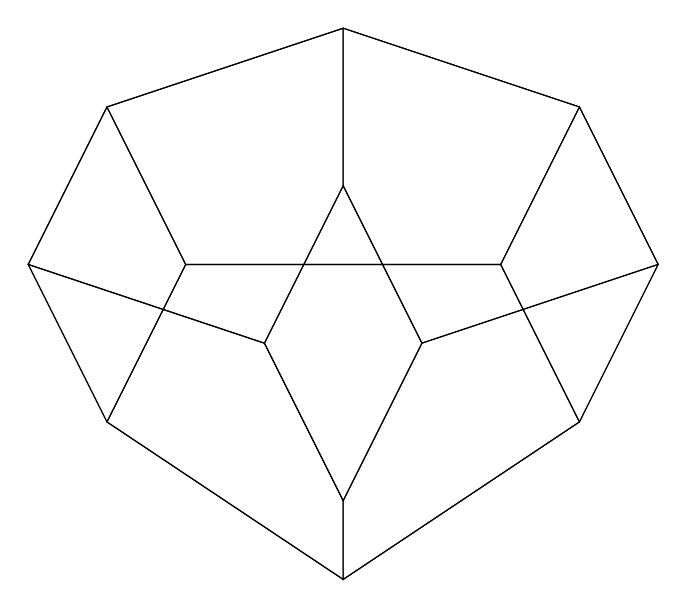
\begin{tikzpicture}[yscale=2]
\coordinate (S11) at (1,0);
\coordinate (S12) at (0,-1);
\coordinate (S13) at (-1,0);
\coordinate (S14) at (0,1);

\coordinate (S21) at (4,0.5);
\coordinate (S22) at (3,-0.5);
\coordinate (S23) at (2,0.5);
\coordinate (S24) at (3,1.5);

\coordinate (S31) at (-2,0.5);
\coordinate (S32) at (-3,-0.5);
\coordinate (S33) at (-4,0.5);
\coordinate (S34) at (-3,1.5);

\coordinate (T) at (0,2);
\coordinate (B) at (0,-1.5);


\draw (S11) -- (S12) -- (S13) -- (S14) -- cycle;
\draw (S21) -- (S22) -- (S23) -- (S24) -- cycle;
\draw (S31) -- (S32) -- (S33) -- (S34) -- cycle;

\draw (T) -- (S14) -- (S13) -- (S33) -- (S34) -- cycle;
\draw (T) -- (S14) -- (S11) -- (S21) -- (S24) -- cycle;
\draw (T) -- (S34) -- (S31) -- (S23) -- (S24) -- cycle;
\draw (B) -- (S32) -- (S31) -- (S23) -- (S22) -- cycle;
\draw (B) -- (S12) -- (S11) -- (S21) -- (S22) -- cycle;
\draw (B) -- (S12) -- (S13) -- (S33) -- (S32) -- cycle;

\end{tikzpicture}

\begin{tikzpicture}[thick,scale=5]
\coordinate (A1) at (0,0);
\coordinate (A2) at (0.6,0.2);
\coordinate (A3) at (1,0);
\coordinate (A4) at (0.4,-0.2);
\coordinate (B1) at (0.5,0.5);
\coordinate (B2) at (0.5,-0.5);

\begin{scope}[thick,dashed,,opacity=0.6]
\draw (A1) -- (A2) -- (A3);
\draw (B1) -- (A2) -- (B2);
\end{scope}
\draw[fill=cof,opacity=0.6] (A1) -- (A4) -- (B1);
\draw[fill=pur,opacity=0.6] (A1) -- (A4) -- (B2);
\draw[fill=greeo,opacity=0.6] (A3) -- (A4) -- (B1);
\draw[fill=greet,opacity=0.6] (A3) -- (A4) -- (B2);
\draw (B1) -- (A1) -- (B2) -- (A3) --cycle;
\end{tikzpicture}

\newdimen\R
\R=0.8cm

\begin{tikzpicture}
\coordinate (P1) at (45:\R);
\coordinate (P2) at (90:\R);
\coordinate (P3) at (135:\R);
\coordinate (P4) at (180:\R);
\coordinate (P5) at (225:\R);
\coordinate (P6) at (270:\R);
\coordinate (P7) at (315:\R);
\coordinate (P8) at (359:\R);
\draw (P1) -- (P2) -- (P3) -- (P4) -- (P5) -- (P6) -- (P7) -- (P8) -- cycle;
\draw[color=red] (P1) -- (P2) -- (P3) -- (P4) -- (P5) -- cycle;
\end{tikzpicture}


\end{document}
